\documentclass[12pt]{article} % use larger type; default would be 10pt
\usepackage[czech]{babel}
\usepackage[utf8]{inputenc} % set input encoding (not needed with XeLaTeX)

%%% PAGE DIMENSIONS
\usepackage{geometry} % to change the page dimensions
% \usepackage[left=2cm,right=2cm,top=2cm,bottom=2cm]{geometry}
\geometry{a4paper}
% \geometry{margin=2in} % for example, change the margins to 2 inches all round
% \geometry{landscape} % set up the page for landscape

\usepackage{graphicx} % support the \includegraphics command and options
\usepackage{wrapfig} % support the wrapfigure section

\usepackage{hyperref} % links in \tableofcontents
\hypersetup{
	colorlinks,
	citecolor=black,
	filecolor=black,
	linkcolor=black,
	urlcolor=black
}

% \usepackage[parfill]{parskip} % Activate to begin paragraphs with an empty line rather than an indent

%%% PACKAGES
\usepackage{booktabs} % for much better looking tables
\usepackage{array} % for better arrays (eg matrices) in maths
%\usepackage{paralist} % very flexible & customisable lists (eg. enumerate/itemize, etc.)
\usepackage{verbatim} % adds environment for commenting out blocks of text & for better verbatim
\usepackage{subfig} % make it possible to include more than one captioned figure/table in a single float
% These packages are all incorporated in the memoir class to one degree or another...
\usepackage{tikz} % graphs
\usepackage{pgfplots}
\usepackage{float}

%%% HEADERS & FOOTERS
\usepackage{fancyhdr} % This should be set AFTER setting up the page geometry
\pagestyle{fancy} % options: empty , plain , fancy
\renewcommand{\headrulewidth}{0pt} % customise the layout...
\lhead{}\chead{}\rhead{}
\lfoot{}\cfoot{\thepage}\rfoot{}

%%% SECTION TITLE APPEARANCE
\usepackage{sectsty}
\allsectionsfont{\sffamily\mdseries\upshape} % (See the fntguide.pdf for font help)
% (This matches ConTeXt defaults)

%%% ToC (table of contents) APPEARANCE
\usepackage[nottoc,notlof,notlot]{tocbibind} % Put the bibliography in the ToC
\usepackage[titles,subfigure]{tocloft} % Alter the style of the Table of Contents
\renewcommand{\cftsecfont}{\rmfamily\mdseries\upshape}
\renewcommand{\cftsecpagefont}{\rmfamily\mdseries\upshape} % No bold!
\newcommand{\bigsize}{\fontsize{35pt}{20pt}\selectfont}

%%% END Article customizations

\begin{document}
\begin{titlepage}
	
\includegraphics[scale=0.7]{logo.jpg}
	\vspace*{\fill}
	\begin{center}
		\textsc{\LARGE Měření činitele zkreslení}\\[1cm]
		Martin Zlámal \\[1cm]
		{\small\em \ Datum měření 3. prosince 2013 } \\
		{\small\em \copyright \ Datum poslední revize \today } \\
		\LaTeX
	\end{center}
	\vspace*{\fill}
\end{titlepage}
%\tableofcontents
%\listoffigures
%\listoftables
\newpage

\section{Zadání}
\begin{enumerate}
\item Seznamte se s principem a ovládáním měřiče zkreslení BM543.
\item Pro jednotlivé polohy nastavovacího prvku zdroje zkreslení ZZ změřte velikost
neharmonického zkreslení (THD).
\item Závislost zkreslení nastavení přepínače zdroje zkreslení ZZ vyneste do grafu.
\end{enumerate}

\section{Schéma zapojení}
\begin{figure}[H]
\center
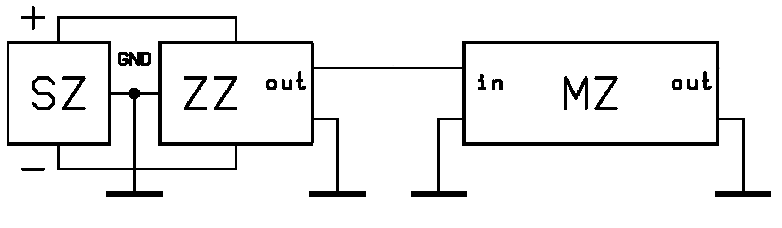
\includegraphics[scale=0.6]{schema.png}
\caption{Reálné schéma zapojení}
\end{figure}

\section{Naměřené a vypočítané hodnoty}
\begin{table}[H]
\caption{Naměřené hodnoty}
\begin{tabular}{|c|c|c|c|c|c|c|c|c|c|c|c|c|}
\hline 
přepínač & $1$ & $2$ & $3$ & $4$ & $5$ & $6$ & $7$ & $8$ & $9$ & $10$ & $11$ & $12$ \\ 
\hline 
$THD\,[\%]$ & $0,0009$ & $0,01$ & $0,05$ & $0,16$ & $0,4$ & $0,82$ & $1,7$ & $3,5$ & $6,2$ & $12$ & $18$ & $32$ \\ 
\hline 
$U\,[V]$ & $2,2$ & $2,9$ & $3,0$ & $3,0$ & $3,1$ & $3,15$ & $3,2$ & $3,3$ & $3,4$ & $3,8$ & $4,1$ & $9,6$ \\ 
\hline 
\end{tabular} 
\end{table}

Ačkoliv v původním zadání byl osciloskop, při reálném měření však nebyl k dispozici, takže jsem tuto část vypustil.

Při měření byl na měřiči zkreslení většinou zapnut automatický způsob meření zkreslení, protože ručně nebylo možné dosáhnout natolik přesných výsledků. Toto platí pouze pro měření zkreslení. Při měření napětí a nastavování $100\%$ rozsahu byl měřící přístroj přepnut do ručního módu.

\section{Grafy}
\begin{figure}[H]
\centering
	\begin{tikzpicture}			
		\begin{axis}[
			width=1\textwidth,
	     	height=0.4\textwidth,
			xlabel={poloha přepínače ZZ},
			ylabel={$THD\,[\%]$}
		]
			
		\addplot coordinates {
			(1,0.0009)
			(2,0.01)
			(3,0.05)
			(4,0.16)
			(5,0.40)
			(6,0.82)
			(7,1.70)
			(8,3.50)
			(9,6.20)
			(10,12.0)
			(11,18.0)
			(12,32.0)
		};
		
		\end{axis}
	\end{tikzpicture}
	\caption{Závislost zkreslení nastavení přepínače zdroje zkreslení ZZ}
\end{figure}

\section{Závěr}
Velikost měřeného zkreslení v závislosti na poloze přepínače zdroje zkresleného signálu stoupá a to kvadraticky. Tato charakteristika svědčí o tom, že na každém rozsahu přepínače vzrostla kvadraticky míra zkreslení oproti původnímu signálu. Číselně je toto zkreslení vyjádřeno v tabulce v procentech.

\section{Přístroje}
\begin{itemize}
\item Stabilizovaný zdroj $\pm$15V/0,5A, evid. 117243
\item Zdroj zkresleného signálu, evid. 117248
\item Měřič zkreslení Tesla BM543, evid. 107616
\end{itemize}

\end{document}
